% To je predloga za poročila o domačih nalogah pri predmetih, katerih
% nosilec je Tomaž Curk. Avtor predloge je Blaž Zupan.
%
% Seveda lahko tudi dodaš kakšen nov, zanimiv in uporaben element,
% ki ga v tej predlogi (še) ni. Več o LaTeX-u izveš na
% spletu, na primer na http://tobi.oetiker.ch/lshort/lshort.pdf.
%
% To predlogo lahko spremeniš v PDF dokument s pomočjo programa
% pdflatex, ki je del standardne instalacije LaTeX programov.

\documentclass[a4paper,11pt]{article}
\usepackage{a4wide}
\usepackage{fullpage}
\usepackage[utf8x]{inputenc}
\usepackage[slovene]{babel}
\selectlanguage{slovene}
\usepackage[toc,page]{appendix}
\usepackage[pdftex]{graphicx} % za slike
\usepackage{setspace}
\usepackage{color}
\definecolor{light-gray}{gray}{0.95}
\usepackage{listings} % za vključevanje kode
\usepackage{hyperref}
\renewcommand{\baselinestretch}{1.2} % za boljšo berljivost večji razmak
\renewcommand{\appendixpagename}{Priloge}

\lstset{ % nastavitve za izpis kode, sem lahko tudi kaj dodaš/spremeniš
language=Python,
basicstyle=\footnotesize,
basicstyle=\ttfamily\footnotesize\setstretch{1},
backgroundcolor=\color{light-gray},
}

\title{Priprava podatkov, osnovne statistike, vizualizacija}
\author{Amon Stopinšek (63150273)}
\date{\today}

\begin{document}

\maketitle

\section{Uvod}

V nalogi smo se spoznali s podatkovno zbirko MovieLens 1995-2016. Cilj naloge je
bila uporaba osnovnih veščin podatkovnega rudarjenja: branje podatkov iz
datoteke, priprava in obdelava podatkov ter vizualiacija.

\section{Podatki}

% Če je naloga zasnovana tako, da vključuje analizo izbranih podatkov, v
% tem razdelku opišeš, kakšni so ti podatki in navedeš nekaj osnovnih
% statističnih lastnosti teh podatkov. Slednje vključujejo velikost
% podatkov (na primer število primerov, število in vrsto atributov), delež
% manjkajočih podatkov, opis in porazdelitev vrednosti ciljnih
% spremenljivk, in podobno. Če si podatke pridobil sam, tu opišeš, na
% kakšen način, kje in kako.

Pri nalogi smo uporabili podatkovno zbirko
\href{https://grouplens.org/datasets/movielens/}{Movie Lens}. Za potrebe naloge
smo uporabili le podatke iz datotek movies.csv, ratings.csv in cast.csv.

Datoteka movies.csv vsebuje podatke o 9125 filmov, ki so opisani z id-jem filma,
naslovom in žanri.

V datoteki ratings.csv je 104 000 ocen filmov. Vsaka ocena je predstavljena z
id-jem uporabnika, id-jem filma, oceno in časovno značko.

Cast.csv vsebuje igralsko zasedbo posameznega filma. Podatki so opisani z id-jem
filma in imeni ter priimki igralcev, ki so med seboj ločen z '\textbar'.

\section{Metode}

% Tu opišeš, na kakšen način si rešil nalogo (tehnike in metode, ki si
% jih uporabil). Lahko vključiš tudi zanimiv del programske kode, ki
% si jo morda pri tem razvil ali pa v poročilo dodatno vključiš sliko,
% kot je na primer slika~\ref{slika1}. Vse slike in tabele, ki jih
% vključiš v poročilo, morajo biti navedene v besedilu oziroma se moraš
% na njih sklicati.
%
% \begin{figure}[htbp]
% \begin{center}
% 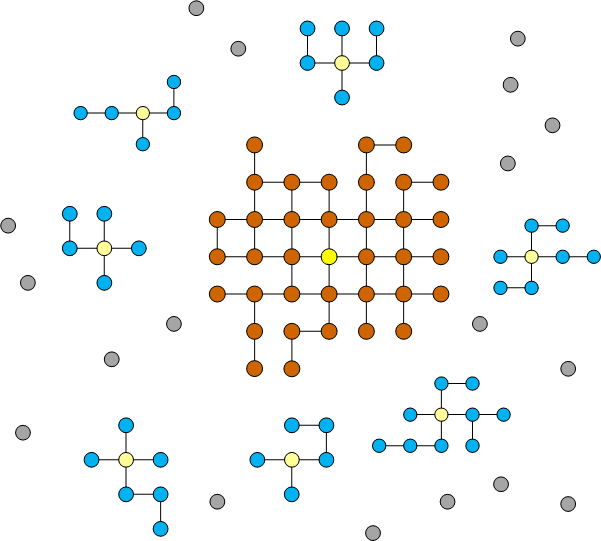
\includegraphics[scale=0.3]{slika-primer.png}
% \caption{Vsako sliko opremi s podnapisom, ki pove, kaj slika prikazuje.}
% \label{slika1}
% \end{center}
% \end{figure}
%
% V to poglavje lahko tudi vključiš kakšen metodološko zanimiv del
% kode. Primer vključitve kode oziroma implementirane funkcije v
% programskem jeziku Python je:
%
% \begin{lstlisting}
% def fib(n):
%     if n == 0:
%         return 0
%     elif n == 1:
%         return 1
%     else:
%         return fib(n-1) + fib(n-2)
% \end{lstlisting}
%
% Izris te kode je lahko sicer tudi lepši, poskušaš lahko najti še
% primernejši način vključevanja kode v Pythonu oziroma v tvojem izbranem
% programskem jeziku v okolje \LaTeX{}.

Za branje podatkov smo uporabil knjižico csv in razred DictReader. Pri branju
podatkov smo le te shranili v slovar. Kot ključ smo najpogosteje uporabili
id filma, za vrednost pa seznam s terkami.
\begin{lstlisting}
reader = DictReader(open('data/ratings.csv', 'rt', encoding='utf-8'))
movieRatings = dict()

for row in reader:
    user = row['userId']
    movie = row['movieId']
    rating = row['rating']
    timestamp = int(row['timestamp'])

    if movie not in movieRatings.keys():
        movieRatings[movie] = []

    movieRatings[movie] = movieRatings[movie] + [(timestamp, float(rating))]
\end{lstlisting}

Za sortiranju podatkov smo uporabili metodi sort() in sorted(), odvisno od
oblike podatkov, ki smo jih želeli urediti.
\begin{lstlisting}
genres = sorted(genres.items(), key=lambda x: x[1])[::-1]
\end{lstlisting}

Pri vizualizaciji smo uporabili knjižico matplotlib. Podatke smo predstavili
z navadnim grafom ali histogramom.
\begin{lstlisting}
plt.figure(figsize=(20, 15))
plt.bar(x, [n for genre, n in genres])
plt.xlim(-0.5, len(genres) - 0.5)
plt.xticks(x)
plt.gca().set_xticklabels([genre for genre, n in genres], rotation=90)
plt.ylabel('Stevilo filmov')
plt.show()
plt.savefig('genres dist.png')
\end{lstlisting}


\section{Rezultati}

% V tem poglavju podaš rezultate s kratkim (enoodstavčnim)
% komentarjem. Rezultate lahko prikažeš tudi v tabeli (primer je
% tabela~\ref{tab1}).

% Odstavke pri pisanju poročila v LaTeX-u ločiš tako, da pred novim
% odstavkom pustiš prazno vrstico. Tudi, če pišeš poročilo v kakšnem
% drugem urejevalniku, morajo odstavki biti vidno ločeni. To narediš z
% zamikanjem ali pa z dodatnim presledkom.
%
% \begin{table}[htbp]
% \caption{Atributi in njihove zaloge vrednosti.}
% \label{tab1}
% \begin{center}
% \begin{tabular}{llp{3cm}}
% \hline
% ime spremenljivke & definicijsko območje & opis \\
% \hline
% cena & [0, 500] & cena izdelka v EUR\\
% teža & [1, 1000] & teža izdelka v dag \\
% kakovost & [slaba|srednja|dobra] & kakovost izdelka \\
% \hline
% \end{tabular}
% \end{center}
% \end{table}
%
% Podajanje rezultati naj bo primerno strukturirano. Če ima naloga več
% podnalog, uporabi podpoglavja. Če bi želel poročati o rezultatih
% izčrpno in pri tem uporabiti vrsto tabel ali grafov, razmisli o
% varianti, kjer v tem poglavju prikažeš in komentiraš samo glavne
% rezultate, kakšne manj zanimive detajle pa vključite v prilogo (glej
% prilogi~\ref{app-res} in~\ref{app-code}).

\subsection{Najbolje povprečno ocenjeni filmi}

\begin{table}[htbp]
\caption{Najbolje povprečno ocenjeni filmi.}
\label{tab1}
\begin{center}
\begin{tabular}{llp{3cm}}
\hline
film & povprečna ocena \\
\hline
Godfather, The (1972) & 4.488 \\
Shawshank Redemption, The (1994) & 4.487 \\
Maltese Falcon, The (1941) & 4.387 \\
Godfather: Part II, The (1974) & 4.385 \\
Usual Suspects, The (1995) & 4.371 \\
Chinatown (1974) & 4.336 \\
Rear Window (1954) & 4.315 \\
12 Angry Men (1957) & 4.304 \\
Schindler's List (1993) & 4.303 \\
City of God (Cidade de Deus) (2002) & 4.297 \\
\hline
\end{tabular}
\end{center}
\end{table}
Pri razvrstitvi filmov po povprečni oceni (prvi poskus~\ref{tab2}) se je pojavil
problem, da so bili najvišje na tej lestvici filmi s samo eno oceno. Problem smo
rešili tako, da smo na lestvico~\ref{tab1} uvrstil le filme z več kot 50 ocenami.

\subsection{Žanri}

\begin{figure}[htbp]
\begin{center}
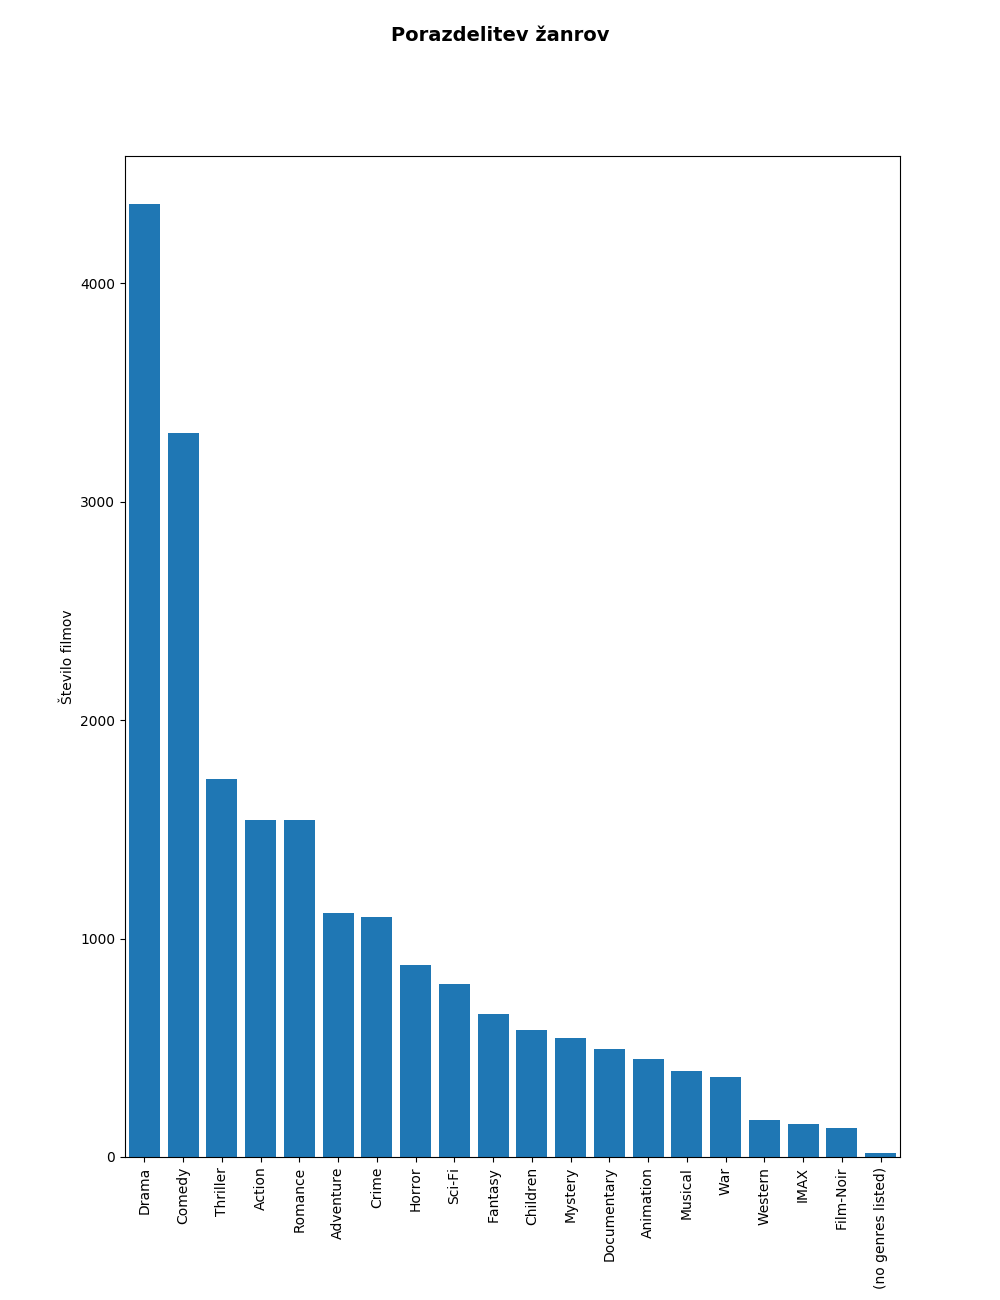
\includegraphics[scale=0.4]{genresDist.png}
\caption{Porazdelitev žanrov po številu filmov} \label{fig:img1}
\end{center}
\end{figure}
Filmi pripadajo 19 oz. 20 (če kot žaner štejemo tudi 'no genres listed') žanrom.
Iz histograma \ref{fig:img1} lahko vidimo, da je najbolj pogost žanr filma drama.


\subsection{Povezava med gledanostjo in povprečno oceno filma}

\begin{figure}[htbp]
\begin{center}
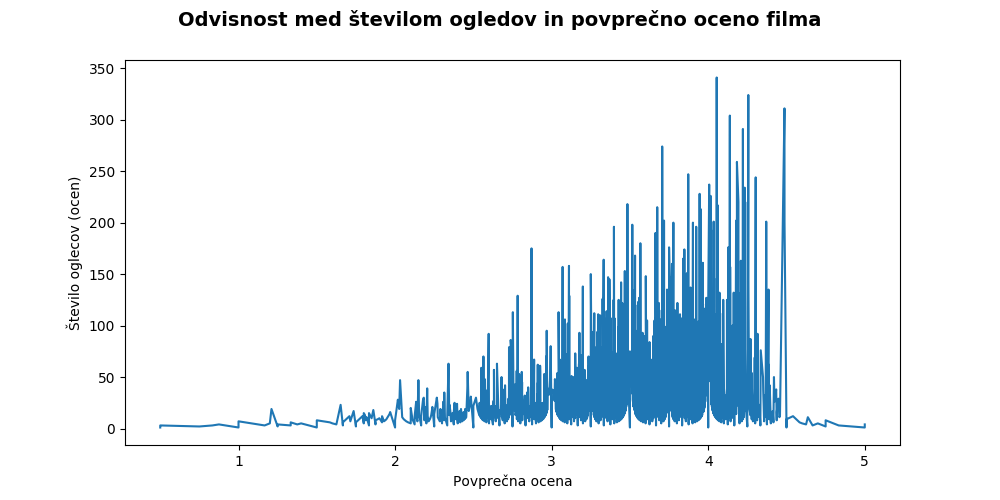
\includegraphics[scale=0.5]{viewsVsMeanRate.png}
\caption{Povezava med povprečno oceno filma in številom ogledov} \label{fig:img2}
\end{center}
\end{figure}
Vizualizacija ~\ref{fig:img2} ni najbolj posrečena, še vseeno pa lahko iz nje
vidimo, da imajo povprečno zelo slabi oz. zelo dobri filmi zelo majhno število
ogledov, običajno pod 25. Če od daleč pogledamo graf lahko vidimo, da imajo filmi
z več ogledi boljšo povprečno oceno (okoli 4), tisti z manj ogledi pa slabšo (
med 2 in 3). Izjema so že omenjeni filmi z malo ogledi in izredno slabo ali dobro
povprečno oceno.

\subsection{Popularnost filmov skozi čas}


\begin{figure}[htbp]
\begin{center}
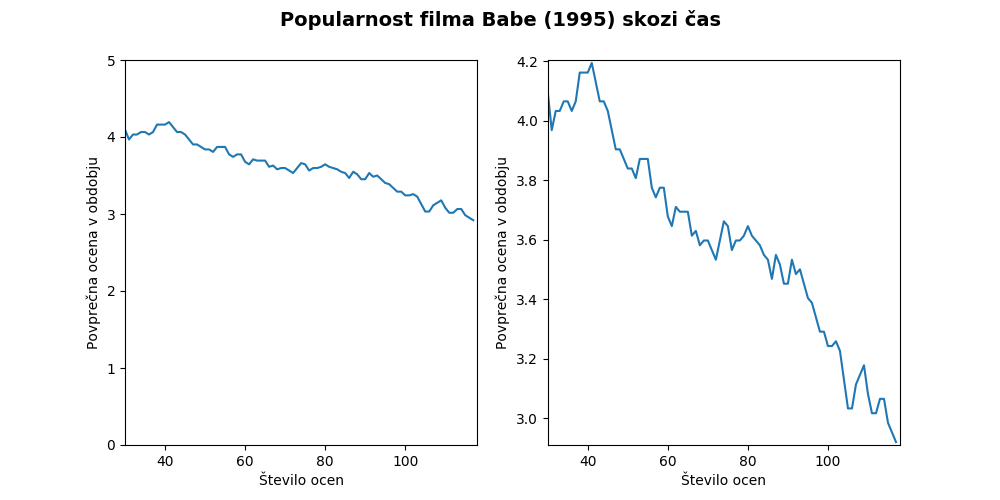
\includegraphics[scale=0.6]{34-babe.png}
\caption{Popularnost filma Babe skozi čas} \label{fig:img4}
\end{center}
\end{figure}

Večina filmov nima velikih skokov v popularnosti skozi čas, če izvzamemo
prvih nekaj ocen. Histogram~\ref{fig:img3} prikazuje, razliko v povprečni
oceni med dvema zaporednima časovnima obdobjema (za dolžino obdobja 30 ocen).
Zanimiva primerka filmov, ki izstopata iz povprečja sta filma Babe~\ref{fig:img4} (povprečna
ocena skozi čas pada iz 4,2 do 2,8) in Beauty and The Beast~\ref{fig:img5} (povprečna
ocena za kratko časovno obdobje skoči za 0,8 in nato pade za več kot 1).


\subsection{Popularnost posameznih igralcev}


\begin{table}[htbp]
\caption{Popularni igralci}
\label{tab3}
\begin{center}
\begin{tabular}{llp{3cm}}
\hline
igralec & ocena popularnosti \\
\hline
Harrison Ford & 9041.5 \\
Tom Hanks & 8426.0 \\
Bruce Willis & 6693.5 \\
Robert De Niro & 6159.0 \\
Morgan Freeman & 6063.0 \\
Brad Pitt & 5516.0 \\
Kevin Spacey & 5172.5 \\
Tom Cruise & 5149.5 \\
Bill Murray & 4903.5 \\
\hline
\end{tabular}
\end{center}
\end{table}

Za izračun popularnosti posameznih igralcev \ref{tab3} smo izbrali preprosto
formulo. Za nastop v filmu smo igralcu k oceni popularnosti prišteli povprečno
oceno filma. Ocena popularnosti igralca je tako sestavljena iz vsote povprečnih
ocen filmov v katerih je nastopal.

\subsection{Najljubši film}
Moj najljubši film je \href{http://www.imdb.com/title/tt0434409/}{V for Vendetta}
Všeč mi je zaradi sporočila ki ga nosi - če se ljudje v dovolj velikem številu
za nekaj združimo in zavzamemo lahko spremenimo svet na bolje. 


\section{Izjava o izdelavi domače naloge}
Domačo nalogo in pripadajoče programe sem izdelal sam.

\appendix
\appendixpage
\section{\label{app-res}Podrobni rezultati poskusov}

\begin{table}[htbp]
\caption{Najbolje povprečno ocenjeni filmi.}
\label{tab2}
\begin{center}
\begin{tabular}{llp{3cm}}
\hline
film & povprečna ocena \\
\hline
Zerophilia (2005) & 5.0 \\
Zelary (2003) & 5.0 \\
Z Channel: A Magnificent Obsession (2004) & 5.0 \\
Yossi (Ha-Sippur Shel Yossi) (2012) & 5.0 \\
Wrong Cops (2013) & 5.0 \\
Wrong (2012) & 5.0 \\
World of Tomorrow (2015) & 5.0 \\
Woman on the Beach (Haebyeonui yeoin) (2006) & 5.0 \\
Woman on Top (2000) & 5.0 \\
Wolf Children (Okami kodomo no ame to yuki) (2012) & 5.0 \\
\hline
\end{tabular}
\end{center}
\end{table}

\begin{figure}[htbp]
\begin{center}
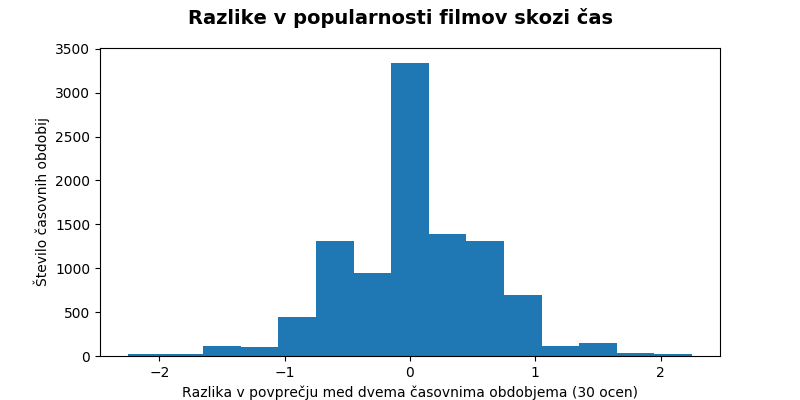
\includegraphics[scale=0.7]{popularityChangesHist.png}
\caption{Sprememba v popularnosti med dvema zaporednima časovnima obdobjema} \label{fig:img3}
\end{center}
\end{figure}

\begin{figure}[htbp]
\begin{center}
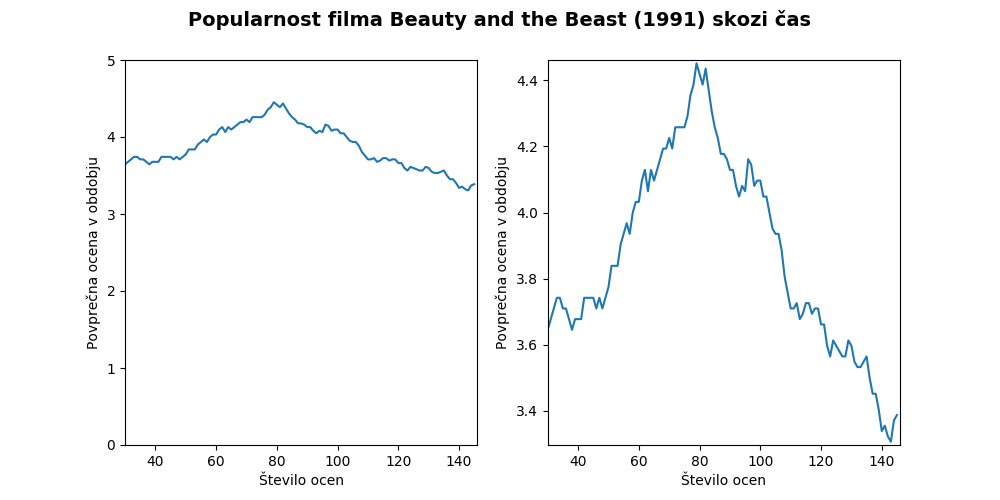
\includegraphics[scale=0.6]{595-beauty.png}
\caption{Popularnost filma Beauty and the Beast skozi čas} \label{fig:img5}
\end{center}
\end{figure}


% \section{\label{app-code}Programska koda}

% Za domače naloge bo tipično potrebno kaj sprogramirati. Celotno kodo oddaj
% zapakirano skupaj s poročilom v datoteki zip. V kolikor je določen izsek kode
% nujen za boljše razumevanje poročila, ga vključi v prilogo poročila.
%
% Čisto
% za okus sem tu postavil nekaj kode, ki uporablja Orange
% (\url{http://www.biolab.si/orange}) in razvrščanje v skupine.
%
%
% \begin{lstlisting}
% import random
% import Orange
%
% data_names = ["iris", "housing", "vehicle"]
% data_sets = [Orange.data.Table(name) for name in data_names]
%
% print "%10s %3s %3s %3s" % ("", "Rnd", "Div", "HC")
% for data, name in zip(data_sets, data_names):
%     random.seed(42)
%     km_random = Orange.clustering.kmeans.Clustering(data, centroids = 3)
%     km_diversity = Orange.clustering.kmeans.Clustering(data, centroids = 3,
%         initialization=Orange.clustering.kmeans.init_diversity)
%     km_hc = Orange.clustering.kmeans.Clustering(data, centroids = 3,
%         initialization=Orange.clustering.kmeans.init_hclustering(n=100))
%     print "%10s %3d %3d %3d" % (name, km_random.iteration, \
%     km_diversity.iteration, km_hc.iteration)
% \end{lstlisting}

\end{document}
